%%%%%%%%%%%%%%%%%%%%%%%%%%%%%%%%%%%%%%%%%
% University Assignment Title Page 
% LaTeX Template
% Version 1.0 (27/12/12)
%
% This template has been downloaded from:
% http://www.LaTeXTemplates.com
%
% Original author:
% WikiBooks (http://en.wikibooks.org/wiki/LaTeX/Title_Creation)
%
% License:
% CC BY-NC-SA 3.0 (http://creativecommons.org/licenses/by-nc-sa/3.0/)
% 
% Instructions for using this template:
% This title page is capable of being compiled as is. This is not useful for 
% including it in another document. To do this, you have two options: 
%
% 1) Copy/paste everything between \begin{document} and \end{document} 
% starting at \begin{titlepage} and paste this into another LaTeX file where you 
% want your title page.
% OR
% 2) Remove everything outside the \begin{titlepage} and \end{titlepage} and 
% move this file to the same directory as the LaTeX file you wish to add it to. 
% Then add \input{./title_page_1.tex} to your LaTeX file where you want your
% title page.
%
%%%%%%%%%%%%%%%%%%%%%%%%%%%%%%%%%%%%%%%%%
%\title{Title page with logo}
%----------------------------------------------------------------------------------------
%   PACKAGES AND OTHER DOCUMENT CONFIGURATIONS
%----------------------------------------------------------------------------------------

\documentclass[14pt]{extarticle}
% \documentclass[bibliography=totocnumbered]{scrartcl}
% \usepackage[english]{babel}
\usepackage[russian]{babel}
\usepackage[utf8x]{inputenc}
\usepackage{float}
\usepackage{amsmath}
\usepackage{graphicx}
\usepackage{subcaption}
\usepackage[colorinlistoftodos]{todonotes}
\renewcommand{\baselinestretch}{1.5}
\usepackage[left=3cm,right=1cm,top=1.5cm,bottom=2cm]{geometry}
\setlength{\parindent}{0mm}
\setlength{\parskip}{1em}
\usepackage{hyperref}
\hypersetup{
    colorlinks,
    citecolor=black,
    filecolor=black,
    linkcolor=black,
    urlcolor=black
}

\begin{document}
\begin{titlepage}

% \newgeometry{margin=2cm}
\newcommand{\HRule}{\rule{\linewidth}{0.5mm}} % Defines a new command for the horizontal lines, change thickness here

\center % Center everything on the page
 
%----------------------------------------------------------------------------------------
%   HEADING SECTIONS
%----------------------------------------------------------------------------------------
\textsc {
\footnotesize{
минобрнауки россии\\
федеральное государственное бюджетное образовательное учреждение\\
высшего профессионального образования}\\
\large{Воронежский государственный университет}
}\\[1.0cm] % Name of your university/college


\textsc{\largeФакультет компьютерных наук}\\ % Major heading such as course name
\textsc{\footnotesize010200 Математика и компьютерные науки}\\[1.0cm] 
\textsc{\Large дипломная работа}\\[0.5cm] % Minor heading such as course title


%----------------------------------------------------------------------------------------
%   TITLE SECTION
%----------------------------------------------------------------------------------------

\HRule \\[0.4cm]
{ \huge \bfseries Ультразвуковой стетоскоп}\\[0.4cm] % Title of your document
\HRule \\[1.5cm]
 
%----------------------------------------------------------------------------------------
%   AUTHOR SECTION
%----------------------------------------------------------------------------------------


\begin{flushleft} \large
\emph{Зав. кафедрой:} С.Д. \textsc{Кургалин}, д. ф-м н., проф.\\
\emph{Студент:} А.А. \textsc{Родионов}, 3 курс, гр 6.1 \\ % Your name
\emph{Руководитель:} Я.А. \textsc{Туровский}, к. мед. н , доцент % Supervisor's Name
\end{flushleft}


% If you don't want a supervisor, uncomment the two lines below and remove the section above
% \Large \emph{Author:}\\
% John \textsc{Smith}\\[3cm] % Your name

%----------------------------------------------------------------------------------------
%   DATE SECTION
%----------------------------------------------------------------------------------------
\vfill % Fill the rest of the page with whitespace
\begin{center}
Воронеж 2017
\end{center}
\end{titlepage}

\tableofcontents
\newpage 
\section{Введение}
Целью данной курсовой работы является создание доступного и простого в производстве цифрового стетоскопа, способного организовать прослушивание легких и сердца человека.

Особенностью данного стетоскопа является то что он может регистрировать сигнал в ультразвуковом диапазоне (до 100 кГц).

В данной работе описывается создание ультразвукогого стетоскопа.

В ходе дипломной работы был создан рабочий прототип прибора. Прибор позволяет получать сигнал от ультразвукового микрофона. Также было написано програмное обеспечение к этому прибору. Програмное обеспечение позволяет позволяет записывать и анализировать звуковые сигналы в реальном времени. Есть возможность рассмотреть различные характеристики сигнала, такие как спектр Фурье, скользящее среднее. Также есть возможность записывать аудиосигнал на жесткий диск для его последующей обработки.

\subsection{Применение прибора на практике}
Устройство планируется использоваться в медицине: анализ ультразвуковой составляющей звука от сердца и легких.

Данный прибор может использоваться в медицине для получения и анализа сигнала высокого качества. Например звук сердца и лёгких. 

Это устройство поможет лучше анализировать звук сердца. С помошью визуализации сигнала можно получить больше информации о звуке внутренних органов, чем простое прослушивание.

Также прибор можно использовать в других областях, где необходим анализ ультразвука. 

Например изучение дельфинов или летучих мышей. 

Сердечно-сосудистые заболевания - самая распространенная причина смерти в мире по данным Всемирной Организации Здравоохранения (ВОЗ). Также распространенными являются заболевания легких. Своевременное наблюдение за состоянием сердца и легких, и обнаружение заболеваний - важная задача здравоохранения.

\newpage  
\section{Описание устройства}
Устройство состоит из нескольких частей, соединенных между собой. От аналогового стетоскопа берется мембрана и соединительная трубка. С одной стороны к соединительной трубке подсоединяется мембрана, с другой - микрофон. Сигнал с микрофона подается на усилитель. С усилителя сигнал подается на Аналогово-Цифровой-Преобразователь (АЦП). Аналогово-Цифровой-Преобразователь подключается к компьютеру через USB-порт.

Мембрана и трубка присоединяется к микрофону для подавления шумов и лучшей передачи звука от сердца/легких. Также усилитель в свою очередь подключается к блоку питания.

\begin{center}
Краткая схема прибора:\\
\noindent\small{{Мембрана → Соединительная Трубка → Микрофон → Усилитель → АЦП → Компьютер}}
\end{center}

% Commands to include a figure:
\begin{figure}[H]
\centering
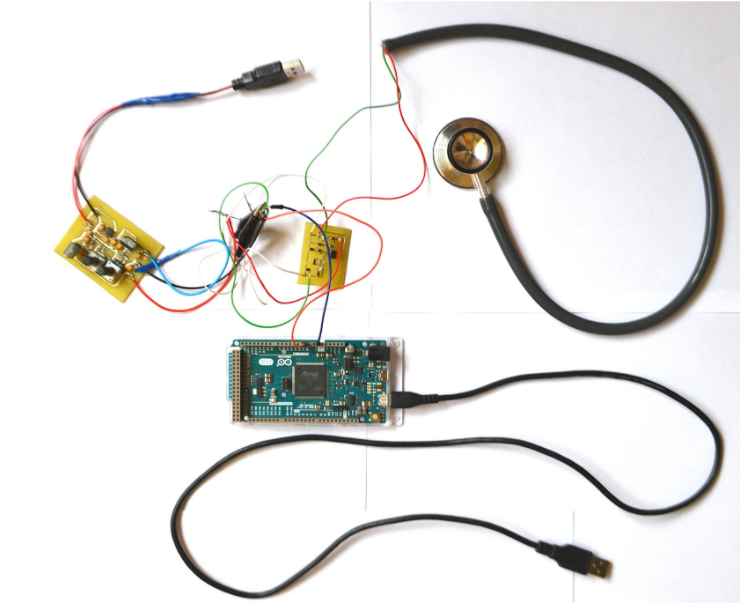
\includegraphics[width=14cm]{hardware.png}
\caption{Собранный прототип}
\end{figure}

\subsection{Технические характеристики деталей стетоскопа}
\subsubsection{Микрофон}
В качестве микрофона был выбран SWEN MK-200. \\

\begin{table}[h]
\centering
\label{my-label}
\begin{tabular}{|l|l|}
\hline
Чувствительность, дБ           & -60 ± 3                    \\ \hline
Диапазон частот, Гц            & 50 – 16 000                \\ \hline
Размер микрофонного модуля, мм & 9×7                        \\ \hline
Тип разъема                    & мини-джек Ø 3,5 мм (3 pin) \\ \hline
Длина кабеля, м                & 1,8                        \\ \hline
Вес, г                         & 63                         \\ \hline
\end{tabular}
\caption{Технические характеристики SWEN MK-200}
\end{table}

Микрофон был вынут из стандартного корпуса, чтобы лучше соединиться с трубкой, ведущей к мембране.

\subsubsection{Усилитель}
Усилитель для микрофона был создан самостоятельно в рамках данной работы.

Была выбрана следующая схема усилителя:

\begin{figure}[H]
\centering
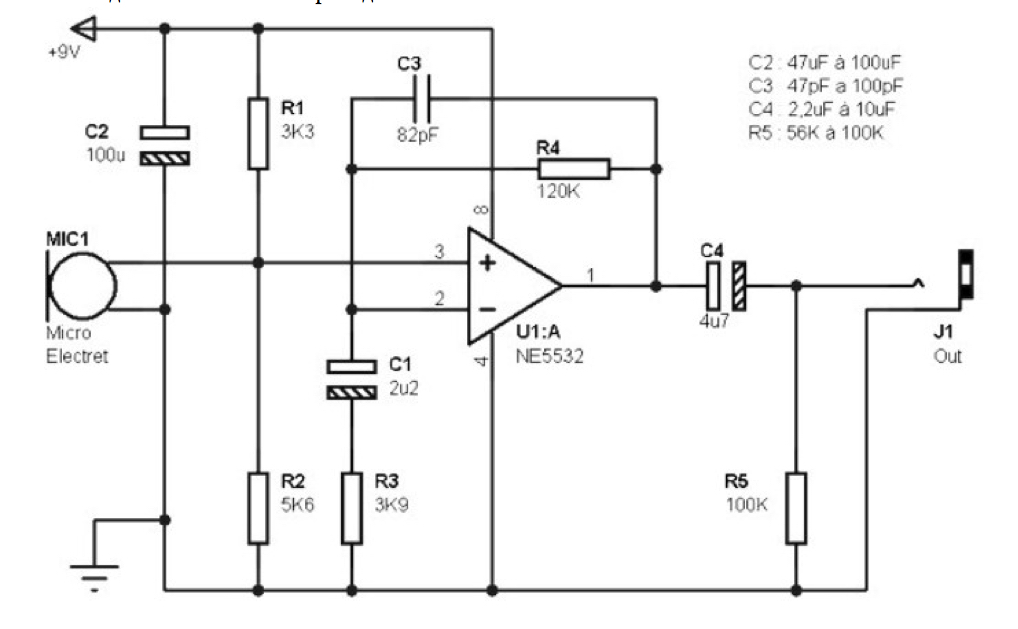
\includegraphics[width=14cm]{circuit.jpg}
\caption{Схема усилителя сигнала}
\end{figure}

В качестве операционного усилителя был выбран \textbf{MCP6022} от производителя Microchip. Это усилитель типа Rail-to-Rail SO-8.

SOIC или просто SO (small-outline-integrated-circuit), а также SOP (Small-Outline Package) корпус микросхем, предназначенный для поверхностного монтажа, занимающий на печатной плате на 30-50\% меньше площади чем аналогичный корпус DIP, а также имеющий на 50-70\% меньшую толщину. Обычно в обозначении также указывается число выводов.

В данный усилитель встроены High-Pass и Low-Pass фильтры. High-Pass фильтрует частоты сигнала меньше 1Гц. Low-Pass фильтрует частоты выше 100кГц. Меняя конденсатор С3, можно менять частоту среза LowPass фильтра. Усиление схемы зависит от резисторов R3 и R4. На текущий момент усиление составляет порядка 100.

Ниже приводятся параметры операционного усилителя.

\begin{table}[h]
\centering
\label{my-label}
\begin{tabular}{|l|l|}
\hline
Полоса частот                  & 10МГц                      \\ \hline
Уровень шума                   & 8.7 нВ/√Гц                 \\ \hline
Количество каналов             & 2                          \\ \hline
Напряжение питания             & 2.5В --- 5.5В              \\ \hline
Напряжение смещения            & $\pm500\mu V $             \\ \hline
Гармонические искажения        & 0.00053\%                  \\ \hline
Температурный диапазон         & -40°C --- +85°C            \\ \hline
Тип корпуса                    & SO-8                       \\ \hline
\end{tabular}
\caption{Технические характеристики операционного усилителя MCP6022}
\end{table}

\begin{figure}[H]
\centering
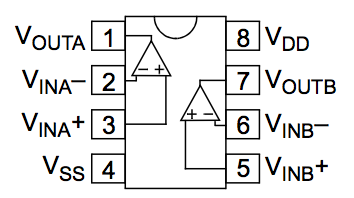
\includegraphics[width=12cm]{op-amp.png}
\caption{Распиновка операционного усилителя}
\end{figure}

\begin{figure}[H]
\begin{subfigure}{0.5\textwidth}
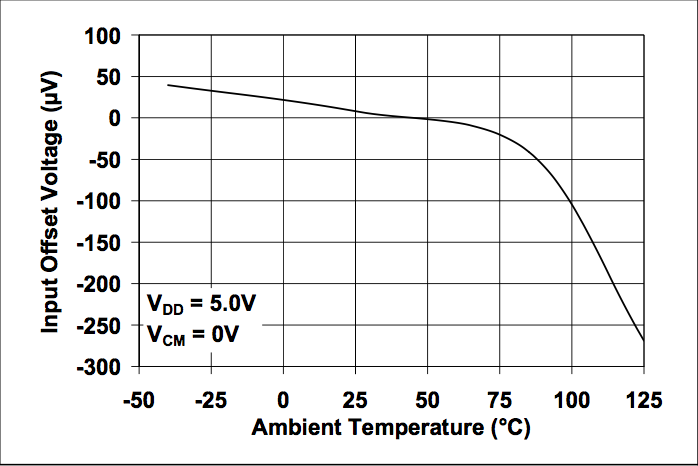
\includegraphics[width=0.9\linewidth, height=5cm]{op-amp-plot1.png} 
\caption{Напряжение смещения --- Температура}
% \label{fig:subim1}
\end{subfigure}
\begin{subfigure}{0.5\textwidth}
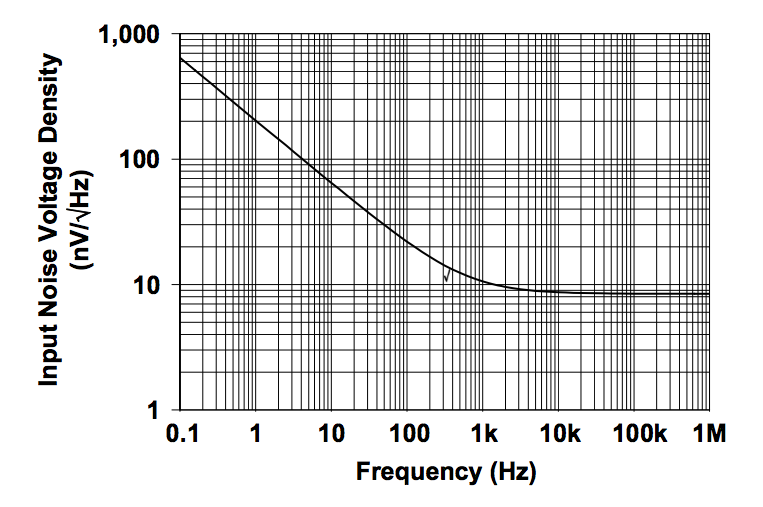
\includegraphics[width=0.9\linewidth, height=5cm]{op-amp-plot2.png}
\caption{Шум --- Частота}
% \label{fig:subim2}
\end{subfigure}

\vspace{10mm} % vertical space
 
\begin{subfigure}{0.5\textwidth}
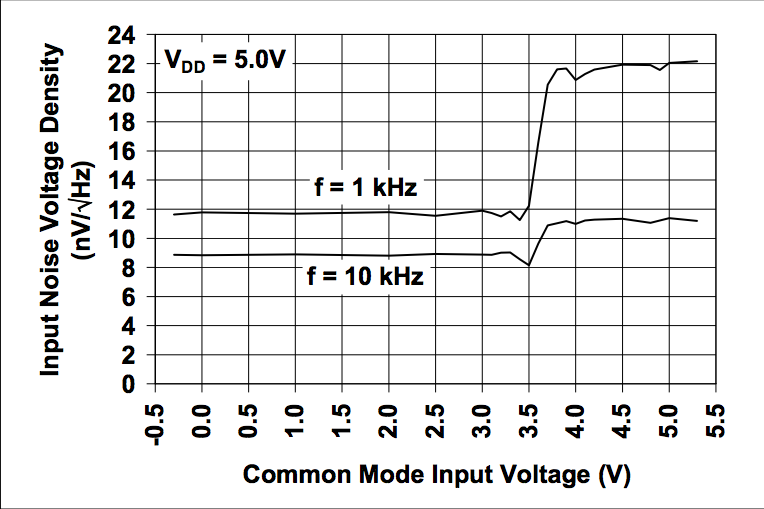
\includegraphics[width=0.9\linewidth, height=5cm]{op-amp-plot3.png} 
\caption{Шум - Напряжение смещения}
% \label{fig:subim1}
\end{subfigure}
\begin{subfigure}{0.5\textwidth}
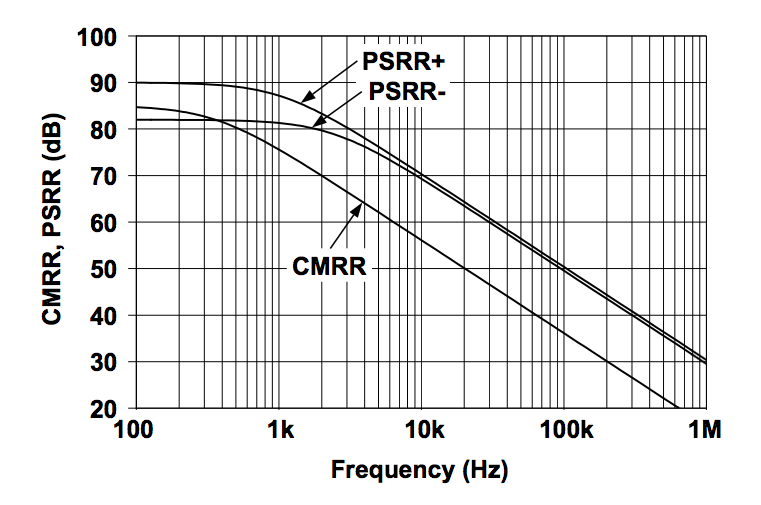
\includegraphics[width=0.9\linewidth, height=5cm]{op-amp-plot4.png}
\caption{CMRR --- Частота}
% \label{fig:subim2}
\end{subfigure}

\vspace{10mm} %vertical space

\begin{subfigure}{0.5\textwidth}
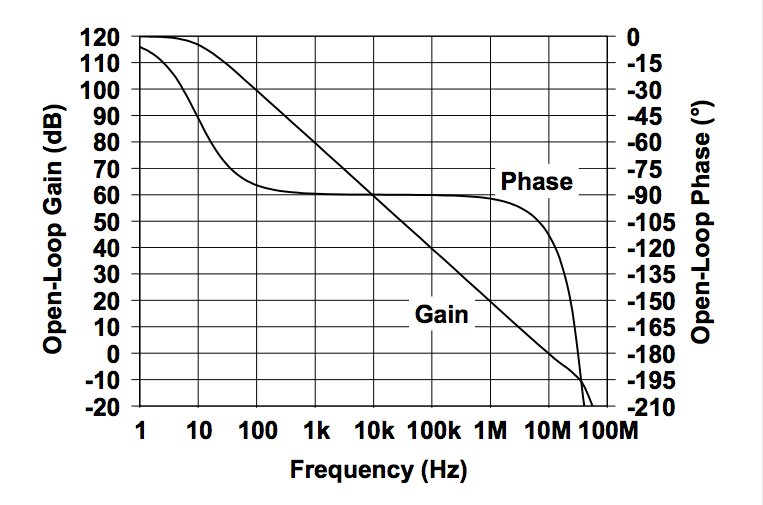
\includegraphics[width=0.9\linewidth, height=5cm]{op-amp-plot5.png} 
\caption{Коэффициент усиления - Частота}
% \label{fig:subim1}
\end{subfigure}
\begin{subfigure}{0.5\textwidth}
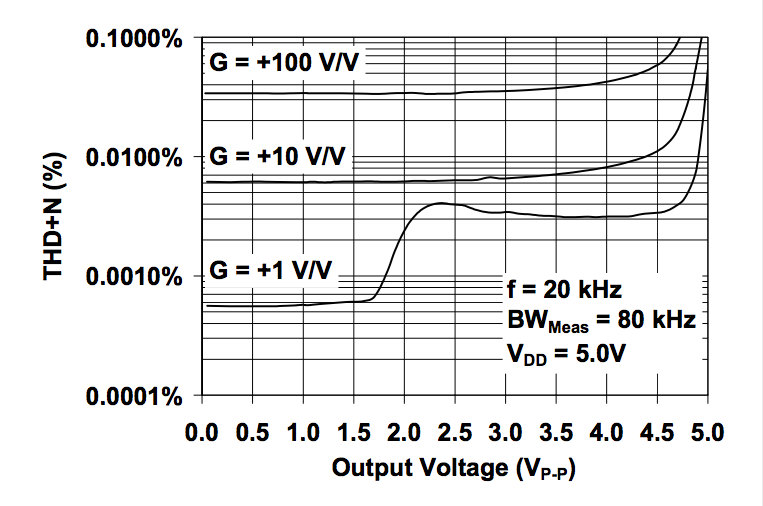
\includegraphics[width=0.9\linewidth, height=5cm]{op-amp-plot6.png}
\caption{\small{Гармонические искажения --- Вых. напряжение (f=20кГц)}}
% \label{fig:subim2}
\end{subfigure}

\caption{Параметры операционного усилителя}
\label{fig:image2}
\end{figure}

Разработка платы усилителя велась в программе Sprint Layout. Ниже представлен скриншот макета платы из этой программы.

\begin{figure}[H]
\centering
% 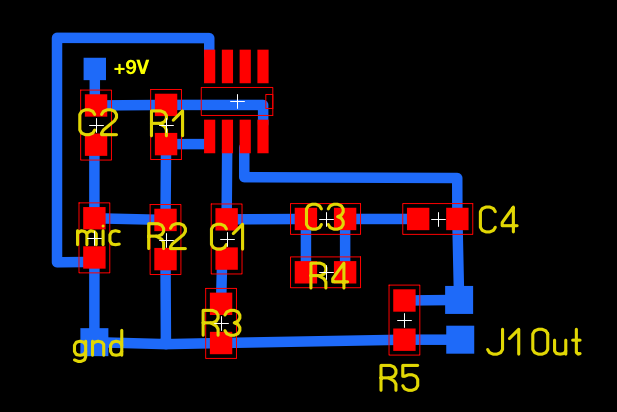
\includegraphics[width=14cm]{sprint-layout-circuit.png}
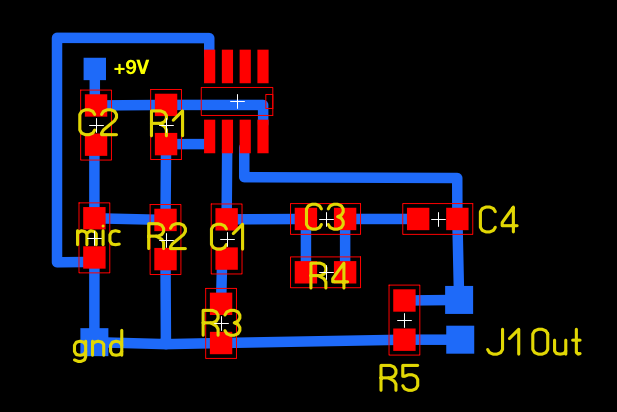
\includegraphics[width=\textwidth]{sprint-layout-circuit.png}
\caption{Схема физической платы усилителя}
\end{figure}

Схема изготавливалась при помощи печати на лазерном принтере методом травления текстолита. 
\subsubsection{АЦП}
В качестве аналого цифрового преобразователя был выбран ЛА-н10-12USB от компании ЗАО "Руднев-Шиляев". Также стетоскоп тестировался на АЦП E-140 от компании LCard. 

Предназначение АЦП – преобразование непрерывных (аналоговых) входных сигналов в цифровую форму для дальнейшей обработки с помощью компьютера.

\begin{table}[h]
\centering
\label{my-label}
\begin{tabular}{|l|l|}
                                                                      \hline
Число аналоговых входов            & 2                             \\ \hline
Минимальная частота дискретизации  & 1.25МГц                       \\ \hline
Максимальная частота дискретизации & 80МГц                         \\ \hline
Объем буффера памяти               & $2\times10^{19}=524288$       \\ \hline
Разрядность                        & 12бит (4096 значений)         \\ \hline
Входное сопротивление              & 50Ом                          \\ \hline
Разъем                             & BNC                           \\ \hline
Диапазоны входного напряжения      & $\pm2V;\pm1V;\pm0.4V;\pm0.2V$ \\ \hline
Защита по входному напряжению      & $\pm5V$                       \\ \hline
Дифференциальная нелинейность      & $\pm1.2$ МЗР                  \\ \hline
Интегральная нелинейность          & $\pm1.5$ МЗР                  \\ \hline
Ошибка сдвига                      & $\pm0.15\%$                   \\ \hline
Интерфейс                          & USB                           \\ \hline
Потребляемая мощность              & 12В, 0.7А                     \\ \hline
Масса                              & 400г                          \\ \hline
\end{tabular}
\caption{Технические характеристики АЦП ЛА-н10-12USB}
\end{table}

\textbf{Интегральная нелинейность} - отклонение по вертикальной оси точек реальной характеристики от идеальной характеристики преобразования, делящих пополам расстояние по оси абцисс между средними значениями пороговых уровней характеристики преобразования. Измеряется в процентах или  МЗР.

\textbf{Дифференциальная нелинейность} - отклонение разности двух аналоговых сигналов от значения, соответствующего единице МЗР.

Данный АЦП работает в режиме старт-стоп. Другими словами он периодически производит запуск, сбор данных(в буффер) и остановку. Это один полный цикл сбора данных. При этом полезное время - это сбор данных, а старт и стоп - бесполезное.

Время, за которое АЦП совершает полный цикл сбора данных и соотношение полезного и бесполезного времени отличается в зависимости от частоты дискретизации и размера буффера. Были произведены замеры времени для различных значений частоты дискретизации и размера буффера и были составлены следующие таблицы.

Во всех таблицах X: размер буффера, Y: частота дискр.

\begin{figure}[H]
\centering
% 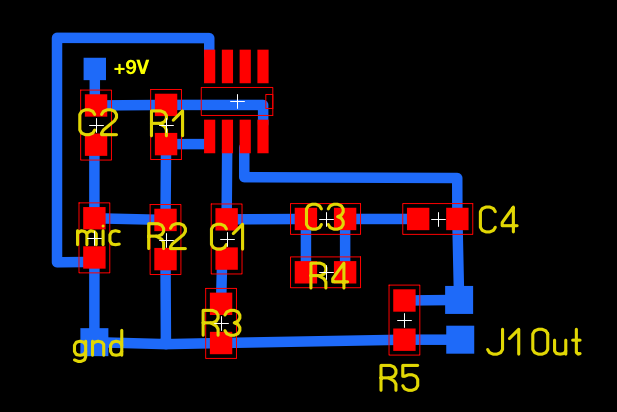
\includegraphics[width=14cm]{sprint-layout-circuit.png}
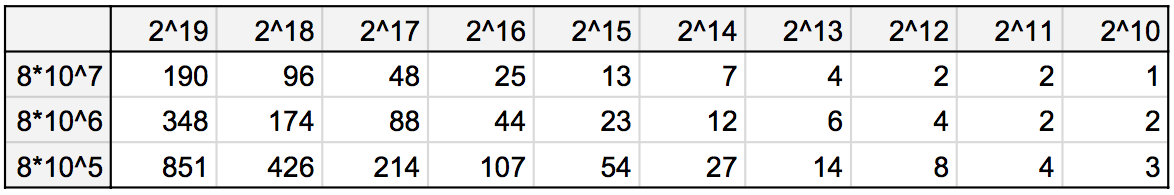
\includegraphics[width=\textwidth]{cycle-time.png}
\caption{Время на полный цикл (мс)}
\end{figure}

\begin{figure}[H]
\centering
% 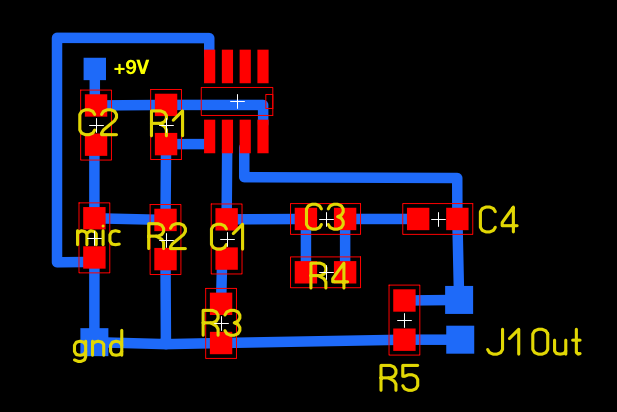
\includegraphics[width=14cm]{sprint-layout-circuit.png}
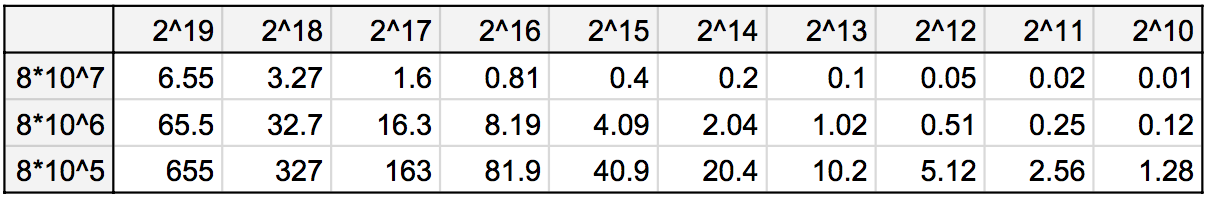
\includegraphics[width=\textwidth]{good-time.png}
\caption{Полезное время (мс)}
\end{figure}

\begin{figure}[H]
\centering
% 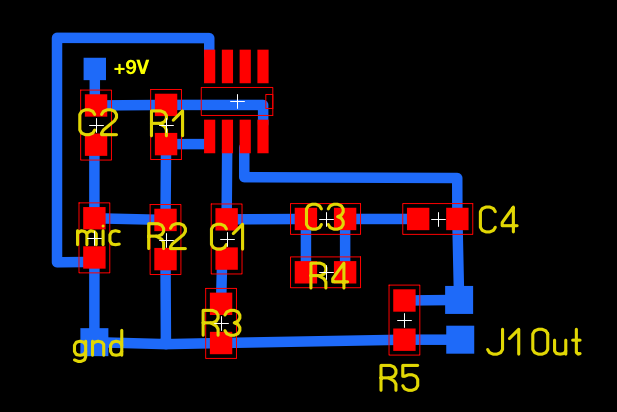
\includegraphics[width=14cm]{sprint-layout-circuit.png}
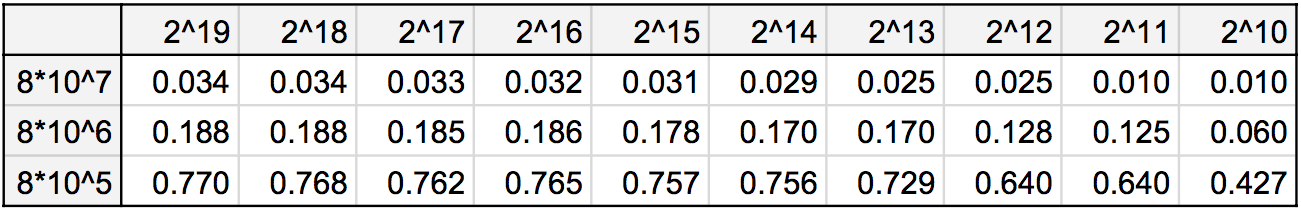
\includegraphics[width=\textwidth]{bad-div-by-good.png}
\caption{Отношение полезного времени к полному}
\end{figure}

\newpage
\section{Описание программного обеспечения}
В рамках данной работы было написано програмное обеспечение для работы с ультразвуковым стетоскопом. Програмное обеспечение написано на языке C\# для платформы Windows.

В функционал програмного обеспечения входит:
\begin{itemize}
  \item Получение сигнала от АЦП ЛА-н10-12USB
  \item Отображение сигнала в реальном времени на экране в виде графика
  \item Отображение спектра сигнала полученного в результате быстрого преобразования Фурье
  \item Отображение скользящего среднего сигнала
  \item Возможность записи сигнала на жесткий диск для последующей обработки
\end{itemize}



\subsection{Инструкция по установке}
\subsection{UI description} with screenshots
\subsection{CUDA Calculations}
\subsection{мб как происходили замеры времени}
\subsection{про параллельность UI / calc}
\subsection{про python version?}
Типа мб написать что в ходе работы над проектом было написано вспомогательное ПО, которое позволяет захватывать звук микрофона, записывать его в wav и анализировать различные параметры, такие как скользящее среднее и спектр сигнала после преобразования фурье.

\subsection{можно добавить как делать запросы к ацп (в программе) Типа узнать MAX-FREQ}


Компьютерная программа для обработки сигнала со стетоскопа написана на языке python c использованием библиотеки pyaudio (для работы со звуком) и библиотеки matplotlib (для визуализации сигналов с помощью графиков)
\subsection{GUI Parameters}
В данном участке кода можно выбрать параметры отображения Графического Интерфейса Пользователя (Graphical User Interface / GUI)
Представлено три параметра:
\begin{verbatim}
timeDomain
freqDomain
lpcOverlay
\end{verbatim}

Каждый из параметров может принимать значение \verb|True| или \verb|False|. В соответсвии с этими параметрами на экране будут(\verb|True|) или не будут(\verb|False|) отображаться соответсвующие элементы.

Параметр \verb|timeDomain| отвечает за отображение звуковой волны. (Зависимость амплитуды сигнала от времени). 

Параметр \verb|freqDomain| отвечает за отображение спектра Фурье звукового сигнала. (Зависимость амплитуды сигнала от частоты). 

Параметр \verb|lpcOverlay| отвечает за отображение усредненного спектра Фурье звукового сигнала. (Апроксимация спектра Фурье многочленами)

\subsection{Stream Parameters}
В данной секции можно настроить параметры захвата аудио с микрофона. Представлено шесть параметров настройки:
\begin{verbatim}
DEVICE
CHUNK
WINDOW
FORMAT
CHANNELS
RATE
\end{verbatim}

Параметр \verb|DEVICE| позволяет выбрать входной порт аудиокарты. Значение этого параметра по умолчанию 0. Если у аудиокарты портов много, то необходимо указать соответсвуующее выбранному  порту значение этого парметра. 

Параметр \verb|CHUNK| - это размер блока сигнала, захватываемого программой за одну итерацию программы. 

Параметр \verb|WINDOW| отвечает за ширину окна программы и количество значений, отображаемых в окне.

Параметр \verb|FORMAT| позволяет выбрать тип данных аудиосигнала. Поддерживаются значения  \verb|paFloat32, paInt32, paInt24, paInt16, paInt8, paUInt8|.

Параметр \verb|CHANNELS| отвечает количество записываемых каналов. Может принимать значения 1 или 2. 

Параметр \verb|RATE| позволяет выбрать частоту дискретизации входного сигнала в Герцах.

\subsection{Spectral parameters}
В данном участке кода представлено два параметра:
\begin{verbatim}
ORDER
NFFT
\end{verbatim}
Параметр \verb|ORDER| отвечает за порядок многочлена, который апроксимирует Фурье-спектр сигнала.

Параметр \verb|NFFT| - размер Фурье спектра по горизонтальной оси.
\subsection{Порядок выполнения программы}
Сначала создается аудиопоток на основе значений Stream Parameters. Затем на основе параметров GUI создаютсе те элементы UI, которые были выбраны пользователем. В этом участке кода можно также уточнить некоторые особенности отображения формы, такие, как наличие сетки (\verb| plt.grid()|) на графике, настройки цвета, количество отображаемых чисел на осях графика. Также можно выбрать границы значений по осям OX и OY для графиков. Также, при необходимости перевести какую-то из осей в логарифмический формат, нужно добавить  соответсвенно строчки:
\begin{verbatim}
plt.xscale('log')
plt.yscale('log')
\end{verbatim}

После инициализации формы с задаными настройками запускается функция анимации: 
\begin{verbatim}
animation = FuncAnimation(fig, update, interval=10)
\end{verbatim}
В параметрах этой функции можно задать временной интервал между кадрами в милисекундах. Функция \verb|animation| запускает функцию \verb|update|. Эта функция обновляет график на каждом кадре анимации. Каждый кадр считывается очередной блок аудиосигнала (\verb|CHUNK|) и на его основе строятся графики, выбранные пользователем. 

Чтобы построить график спектра Фурье сигнала, в функции \verb|spectral_estimate| выполняется преобразование фурье. Для этой цели используется библиотека numpy.

Чтобы построить апроксимированный многочленом спектр Фурье, выполняется функция \verb|lpc_spectrum|.

\newpage
\section{Заключение}
В процессе данной работы был создан рабочий прототип устройства, позволяющего анализировать в реальном времени звуковой сигнал, поступающий от сердца или легких. Данное устройство может применяться для получения дополнительной информации, которую человек не может услышать на обычном стетоскопе.

Сфера применения не ограничена медициной, устройство позволяет анализировать любые типы ультразвуковых сигналов.

Развитие проекта можно продолжить в направлении улучшения качества звука. Для этого нужно использовать более дорогие микрофон и усилитель. Также нужно произвести опрос врачей о том, какие именно характеристики звука со стетоскопа важны.

Улучшений в програмном обеспечении можно достигнуть путем оптимизации алгоритмов распаралеливания на нескольких ядрах процессора или на видеокарте. На основе информации от докторов, можно сделать систему распознавания различных забовалеваний легких и сердца.

Разработка данного проекта велась с помощью системы контроля версий git. Исходный код програмного обеспечения, этапы создания и документация доступны по адресу:

\url{https://github.com/tandav/ultrasonic-stethoscope}

\newpage
\renewcommand\refname{Ссылки на источники}
\begin{thebibliography}{}
\bibitem{latexcompanion} 
Аналого цифровой преобразователь ЛА-н10-12USB\\
\url{http://www.rudshel.ru/show.php?dev=14}

\bibitem{latexcompanion} 
Документация по программированию устройств ЗАО "Руднев-Шиляев"\\
\url{http://www.rudshel.ru/soft/SDK2/Doc/CPP_USER_RU/html/index.html}

\bibitem{latexcompanion} 
Руководство пользователя ЛА-н10-12USB\\
\url{http://www.rudshel.ru/pdf/LA-n10-12USB(y).rar}

\bibitem{latexcompanion} 
Внешний USB АЦП/ЦАП E14-140-M\\
\url{http://www.lcard.ru/products/external/e-140m)}

\bibitem{latexcompanion} 
Схема усилителя для микрофона\\
\url{http://full-chip.net/analogovaya-elektronika/70-usilitel-dlya-elektretnogo-mikrofona-s-nizkim-urovnem-shuma-shema.html}

\bibitem{latexcompanion} 
Руководство пользователя и технические характеристики операционного усилителя MCP6022\\
\url{https://lib.chipdip.ru/291/DOC000291231.pdf}

\bibitem{latexcompanion} 
Исходный код, документация и этапы создания проекта ультразвукового стетоскопа\\
\url{https://github.com/tandav/ultrasonic-stethoscope}

\end{thebibliography}


\end{document}
